\documentclass{beamer}
\beamertemplatenavigationsymbolsempty
\usecolortheme{beaver}
\setbeamertemplate{blocks}[rounded=true, shadow=true]
\setbeamertemplate{footline}[page number]
%
\usepackage[utf8]{inputenc}
\usepackage[english,russian]{babel}
\uselanguage{russian}
\deftranslation[to=russian]{Theorem}{Теорема}
\deftranslation[to=russian]{theorem}{теорема}
\deftranslation[to=russian]{Corollary}{Следствие}
\deftranslation[to=russian]{corollary}{следствие}
% \usepackage[style=verbose, backed=biber]{biblatex}
\usepackage{amssymb,amsfonts,amsmath,mathtext}
\DeclareMathOperator*{\argmax}{arg\,max}
\DeclareMathOperator*{\argmin}{arg\,min}
\usepackage{subfig}
\usepackage[all]{xy} % xy package for diagrams
\usepackage{array}
\usepackage{multicol}% many columns in slide
\usepackage{hyperref}% urls
\usepackage{hhline}%tables
\usepackage{natbib}
\usepackage[labelformat=empty]{caption}
% \usepackage{setspace}
% \usepackage{natbib}
\usepackage{relsize}
\usepackage{blindtext}
\usepackage{doi}
\usepackage{mathtools}
\usepackage{graphicx}
% \usepackage{enumitem}
\usepackage{multirow}
\usepackage{makecell}
\newtheorem{statement}{Утверждение}
\usepackage{etoolbox}
\usepackage{totcount}
% \makeatletter
% \patchcmd{\@makefnmark}
%   {\hbox{\@textsuperscript{\normalfont\@thefnmark}}}
%   {\hbox{\@textsuperscript{\tiny\@thefnmark}}}
%   {}{}
% \makeatother
\newcommand\blfootnote[1]{%
\begingroup
\renewcommand\thefootnote{}\footnote{#1}%
\addtocounter{footnote}{-1}%
\endgroup
}

\newtotcounter{realframenumber}

\setbeamertemplate{footline}{
  \hfill
  \insertframenumber{} / \total{realframenumber}
  \hspace{1em}
}

% Your figures are here:
\graphicspath{ {fig/} {../fig/} }

%----------------------------------------------------------------------------------------------------------
\title[\hbox to 56mm{Индуктивное смещение}]{Выбор предсказательной модели в режиме многозадачного обучения с применением символьных методов}
\author[М.\,Ф. Набиев]{
    Набиев Мухаммадшариф Фуркатович
}
\institute[Московский физико-технический институт]{
\small{
    Московский физико-технический институт \\
    Кафедра интеллектуальных систем ФПМИ МФТИ \\ 
    Научный руководитель: к.ф.-м.н. Бахтеев Олег Юрьевич
}}
\date{2025}
%----------------------------------------------------------------------------------------------------------
\begin{document}
%----------------------------------------------------------------------------------------------------------
\begin{frame}[plain]
\stepcounter{realframenumber}
\thispagestyle{empty}
\maketitle
\end{frame}
%-----------------------------------------------------------------------------------------------------
\begin{frame}{Цель исследования}
\stepcounter{realframenumber}
\textbf{Проблема:} Выбор оптимальной предсказательной модели сильно зависит от априорного знания человека о природе данных, т.е. от их индуктивного смещения. Определение индуктивного смещения автоматическим образом является открытой проблемой.  \\ 
% \newline
\vspace{1mm}
% \begin{spacing}{0.4}
\textit{Примером индуктивного смещения могут служить свертки для изображений и временная зависимость для авторегресии.} \\
% \newline
% \end{spacing}
\vspace{1mm}
% \newline
% \newline 
\textbf{Цель:} Предложить метод автоматического определения индуктивного смещения.
\newline
\newline
\textbf{Решение:} Построение модели в режиме многозадачного обучения с применением символьной регрессии и дальнейшая ее интерпретация.
\end{frame}
%-----------------------------------------------------------------------------------------------------
\begin{frame}{Архитектура решения}
\stepcounter{realframenumber}
\begin{columns}[c]
\column{0.45\textwidth}
\begin{figure}
    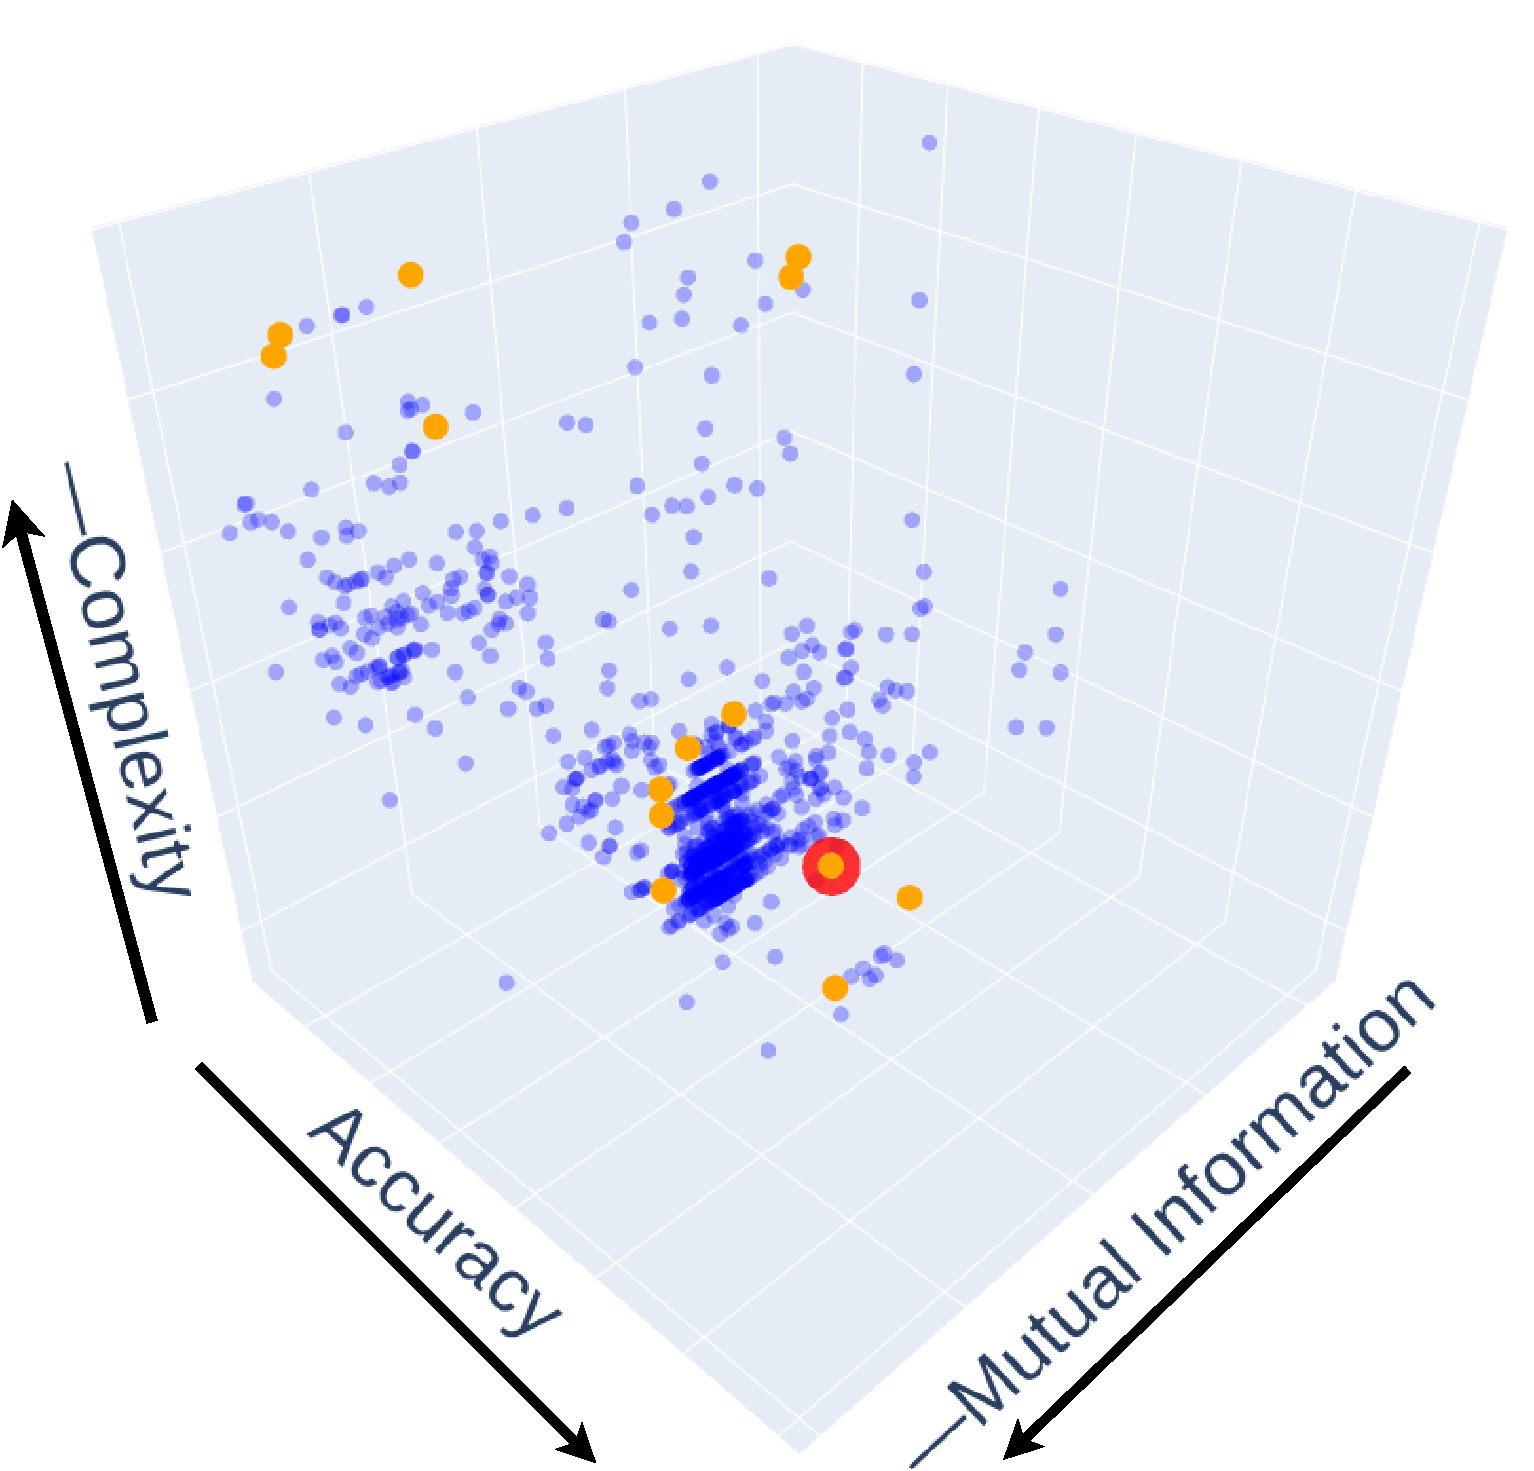
\includegraphics[scale=0.13]{3d_paretto_front.pdf}
    \caption{\scriptsize Модели с искомыми критериями. Оранжевым выделен Парето-фронт, а красным --- истинная модель.}
\end{figure}
\column{0.55\textwidth}
\begin{figure}
    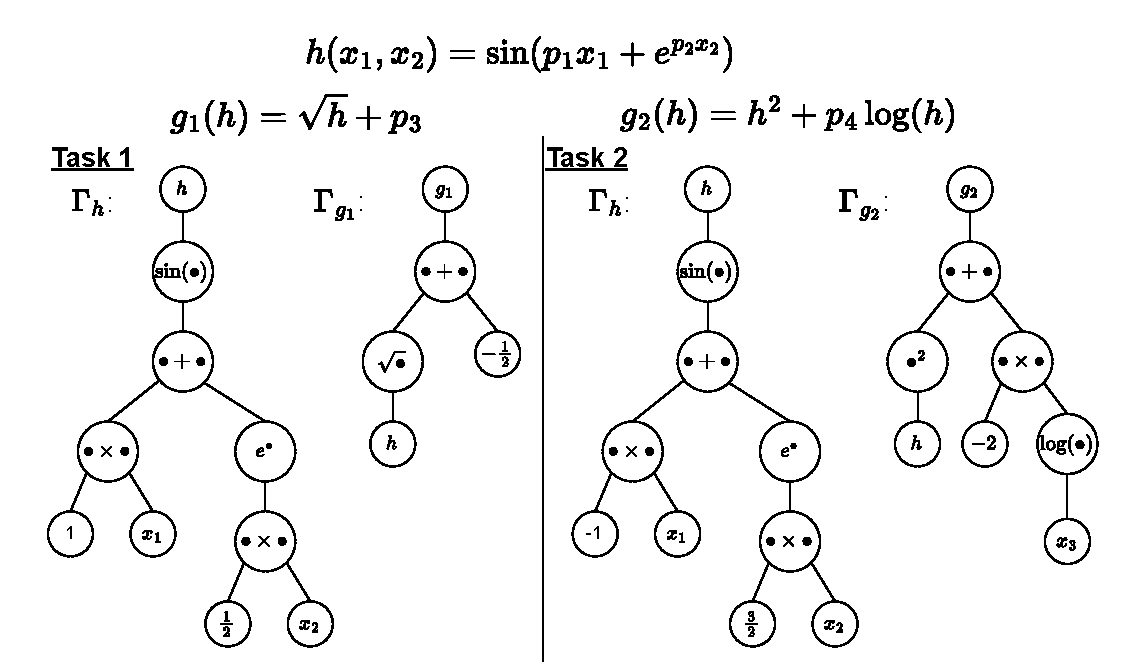
\includegraphics[width=0.9\textwidth]{expression_tree.drawio.pdf}
    \caption{\scriptsize Структура модели в виде дерева разбора.}
\end{figure}
\end{columns}
{\scriptsize \setlength{\baselineskip}{\baselineskip} Предлагается выбирать модель в режиме многозадачного обучения c учетом информационных критериев.\\}\blfootnote{\scriptsize Caruana. Multitask learning: a knowledge-based source of inductive bias. 1993}
% \vspace{2mm}
{\scriptsize \setlength{\baselineskip}{\baselineskip} \textbf{Гипотеза:} модель, отражающая индуктивное смещение, располагается на Парето-фронте по следующим критериям: предсказательная способность, длина описания и взаимная информация между исходным объектом выборки и его представлением.\\}
\end{frame}
%----------------------------------------------------------------------------------------------------------
\begin{frame}{Постановка задачи}
\stepcounter{realframenumber}
Пусть \(\mathfrak{T} = \{T_i\}_{i=1}^m\)~-- множество задач. Задаче \(T_i\) соответствует набор данных \( \mathfrak{D}_i = (\mathbf{X}^i, \mathbf{y}_i) \), где \(\mathbf{X}^i \in \mathbb{R}^{N_i \times n}\),  а \(\mathbf{y}^i \in \mathcal{Y}\). Для регрессии \(\mathcal{Y} =  \mathbb{R}^{N_i}\) а для классификации \(\mathcal{Y} =  \{1, \dots, K\}^{N_i}\).
\begin{itemize}
    \item Моделью \(\mathbf{f}(\mathbf{x}; \mathbf{w})\) назовем отображение \(\mathbb{R}^n \times \mathbb{R}^l \rightarrow \mathcal{Y}^m\), структура \(\Gamma_{\mathbf{f}}\) модели которой представима в виде дерева разбора символьного выражения. 
    \item Декомпозируем модель как \(\mathbf{f} = \mathbf{g} \circ \mathbf{h} = (g_1 \circ \mathbf{h}, \dots, g_m \circ \mathbf{h})\). Модели \(\mathbf{h}\) и \(\mathbf{g}\) мы назовем \textit{энкодером} и \textit{декодером} соответственно.
    \item Назовем \textit{индуктивным смещением} для декомпозируемой модели структуру первой части \(\Gamma_{\mathbf{h}}\) модели \(\mathbf{f}\).
\end{itemize}

\begin{statement}[Набиев, 2025]
    Для любой модели $\mathbf{f}: \mathbb{R}^n \to \mathcal{Y}^m$ существует такая модель $\mathbf{h}: \mathbb{R}^n \to \mathbb{R}^d$ и $\mathbf{g}: \mathbb{R}^d \to \mathcal{Y}^m$, что $f = g \circ h$.
\end{statement}
\end{frame}
%----------------------------------------------------------------------------------------------------------
\begin{frame}{Постановка задачи}
\stepcounter{realframenumber}
\begin{theorem}[Набиев, 2025]
    Для скрытого пространства $\mathbb{R}^d$, такого что $d \geq m$, существует разложение $f = g \circ h$, где $g = \mathrm{Id}_Z$, а $Z \cong \mathcal{Y}^m$.
\end{theorem}
Энкодер \(\mathbf{h}\) задает достаточную статистику относительно \(\mathbf{y}\), если \(\operatorname{I}(\mathbf{h}(\mathbf{X}), \mathbf{y}) = \operatorname{I}(\mathbf{X}, \mathbf{y})\). \\ \textbf{Принцип Information Bottleneck (IB)}\blfootnote{\scriptsize Tishby, Zaslavsky. Deep learning and the
information bottleneck principle. 2015} --- приближение минимальной достаточной статистики: \vspace{-10}
$$
\min_{p(\mathbf{h}(\mathbf{x})\mid \mathbf{x})} \operatorname{I}(\mathbf{X}, \mathbf{h}(\mathbf{X})) - \beta \operatorname{I}(\mathbf{h}(\mathbf{X}), \mathbf{y}), \vspace{-10}
$$
где параметр $\beta$ задаёт баланс между сжатием и значимостью. Для выполнения условия достаточности минимизируем $\operatorname{I}(\mathbf{X}, \mathbf{h}(\mathbf{X}))$: \vspace{-10}
$$
\operatorname{I}(\mathbf{X}, \mathbf{h}(\mathbf{X})) - \beta \operatorname{I}(\mathbf{h}(\mathbf{X}), \mathbf{y}) \approx \operatorname{I}(\mathbf{X}, \mathbf{h}(\mathbf{X})) - \beta^{\prime} \cdot L(f_i(\mathbf{X}), \mathbf{y}), \vspace{-10}
$$
где $L$ — функция потерь.

\end{frame}
%----------------------------------------------------------------------------------------------------------
\begin{frame}{Постановка задачи}
\stepcounter{realframenumber}
Задача оптимизации принимает вид: \vspace{-5}
\begin{align*}
    \Gamma_{\mathbf{h}} = &\; \argmin_{\mathbf{f} = (\mathbf{g}_1 \circ \mathbf{h}, \dots, \mathbf{g}_m \circ \mathbf{h})} 
    \frac{1}{m} \sum_{i=1}^m L_i(f_i(\mathbf{X}^i; \mathbf{w}^*_i), \mathbf{y}^i) + \lambda_1\operatorname{I}(\mathbf{X}^i, \mathbf{h}(\mathbf{X}^i))+ \lambda_2C(\mathbf{f}),\\ 
    & \text{s.t.} \; 
    \mathbf{w}^*_i = \argmin_{\mathbf{w}} L_i(f_i(\mathbf{X}^i; \mathbf{w}), \mathbf{y}^i)
\end{align*}
{\small где \(\operatorname{C}: \mathfrak{F} \rightarrow \mathbb{R}\) --- длина описания модели, с помощью кодирования Хаффмана.}
\begin{theorem}[Набиев, 2025]
Пусть кол-во задач $m=1$. Тогда существует решение $f$, которое можно разложить как $f = g \circ h$, где $g = \operatorname{Id}$, а $h = f$.
\end{theorem} \vspace{-5}
\begin{corollary}
Пусть имеется $m > 1$ задач, и пусть каждая задача $T_i$ аппроксимируется функцией $ f_i(\mathbf{x}) = \left[ \mathbf{f}(\mathbf{x}, \mathbf{w}_i) \right]_i, $ где: $\Gamma_{g_i} = \Gamma_{g_j}$ для всех $i, j \in \{1, \dots, m\}$. Тогда существует декомпозиция вида $ \mathbf{h}(\mathbf{x}, \mathbf{w}) = \mathbf{f}(\mathbf{x}; \mathbf{w}), \quad \mathbf{g}(\mathbf{x}) = \mathbf{x},$ такая что для каждой задачи $ f_i(\mathbf{x}) = (\mathbf{g} \circ \mathbf{h})(\mathbf{x}; \mathbf{w}_i) = \mathbf{h}(\mathbf{x}; \mathbf{w}_i)$.
\end{corollary}

\end{frame}
%----------------------------------------------------------------------------------------------------------
\begin{frame}{Данные для эксперимента}
\stepcounter{realframenumber}
Эксперимент проводился на четырех типах выборок:
\begin{enumerate}
    \item \textbf{Окружность}: 3 задачи: данные --- точки окружности. Задачи имеют вид: \([r > 0], r + 0.5\) и \(\sqrt{r} - 0.5\). Оптимальная модель --- кривая второго порядка.
    \item \textbf{Авторегрессия}: Задачи вида: \(y_t = \alpha y_{t-1} + \varepsilon\). Модели оценивались по взаимной информации и длине описания.
    \item \textbf{4-пикселя}: 8 задач: 6 бинарных классификаций и 2 регрессии. Оптимальная модель --- использует локальную пространственную информацию.
    \item \textbf{MNIST}: Сравнивались модели с масками, имитирующими свёртки, и случайными масками.
\end{enumerate}
\textbf{Гипотеза:} структура энкодера будет содержать операции характерные для заданного типа выборки.
\end{frame}
%----------------------------------------------------------------------------------------------------------
\begin{frame}{Результаты эксперимента: окружность и 4-пикселя}
\stepcounter{realframenumber}
\begin{columns}[c]
\column{0.7\textwidth}
Окружность: 
\begin{enumerate}
    \itemsep0em 
    \item \({\scriptstyle h_0 = p_1, \; h_1 = x_0^2 + x_1^2}\)
    \item \({\scriptstyle h_0 = (p_2x_0 + x_1)^2, \; h_1 = p_1}\)
    \item \({\scriptstyle h_0 = x_0^2 + x_1^2, \; h_1 = p_0}\)
    \item \({\scriptstyle h_0 = p_2, \; h_1 = (x_1 + p_0x_0)^2}\)
    \item \({\scriptstyle h_0 = (x_0 + x_1)^2, \; h_1 = p_2}\)
\end{enumerate}
\textbf{\scriptsize Вывод:} {\scriptsize \setlength{\baselineskip}{0.8\baselineskip} Модели 1, 3 и 5 демонстрируют высокую точность при минимальной сложности, соответствуя структуре задачи, а 2 и 4 не доминируют.\\}
\noindent
\rule{\linewidth}{0.4pt}
4-пикселя:
\begin{enumerate}
    \itemsep0em
    \item \({\scriptstyle h_0 = p_3x_1 - x_0  -x_2 - p_5, \; h_1 = p_2x_2 + x_3}\)
    \item \({\scriptstyle h_0 = x_1, \; h_1 = \max(p_4, x_2-x_0) + p_5x_2 - x_3}\)
    \item \({\scriptstyle h_0 = (x_1+p_2)(p_3x_3 + p_1x_2), \; h_1 = x_1 + p_1x_0}\)
    \item \({\scriptstyle h_0 = p_3x_1 - x_3(p_0 + x_2), \; h_1 = x_0 + p_2x_2}\)
    \item \({\scriptstyle h_0 = p_3(x_2 - p_4)(p_2 + x_0 + x_1), \; h_1 = x_1(p_1 - x_3)}\)
\end{enumerate}
\textbf{\scriptsize Вывод:} {\scriptsize \setlength{\baselineskip}{0.8\baselineskip} Все модели, кроме 2, локальны (учитывает пиксель и соседей в радиусе 2) и хорошо сбалансированы по точности, длине описания и взаимной информации.\\}
\column{0.3\textwidth}
\begin{figure}
    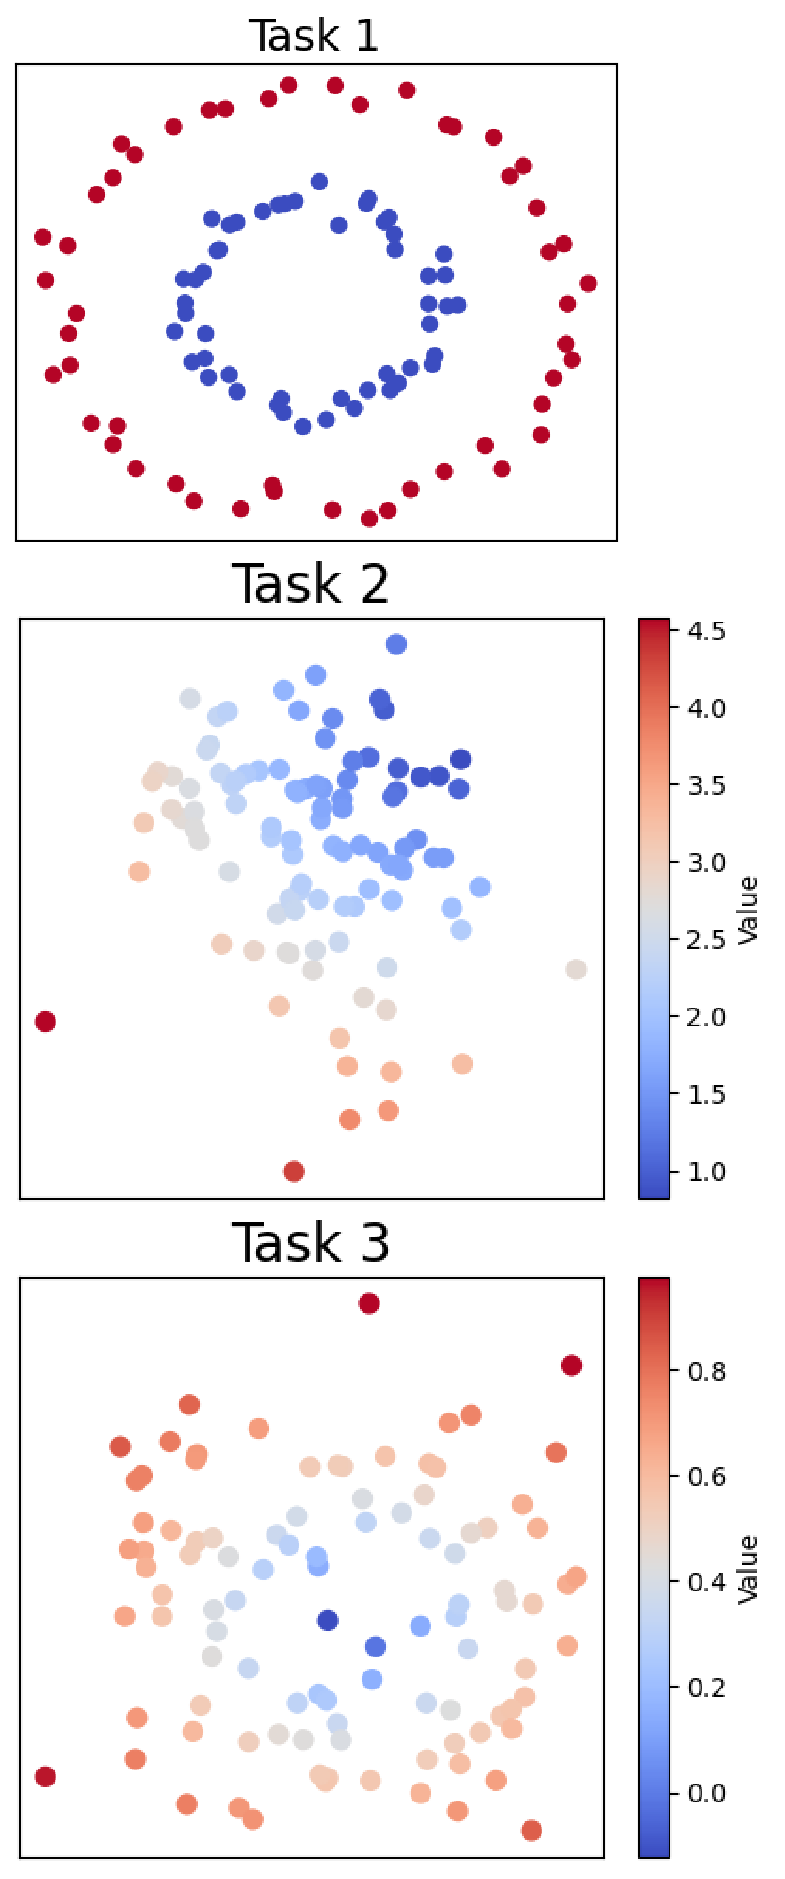
\includegraphics[scale=0.23]{circles.drawio.pdf}
    % \caption{\scriptsize Задачи.}
\end{figure}
\end{columns}
\end{frame}
%----------------------------------------------------------------------------------------------------------
\begin{frame}{Результаты эксперимента: MNIST}
\stepcounter{realframenumber}
\begin{figure}
    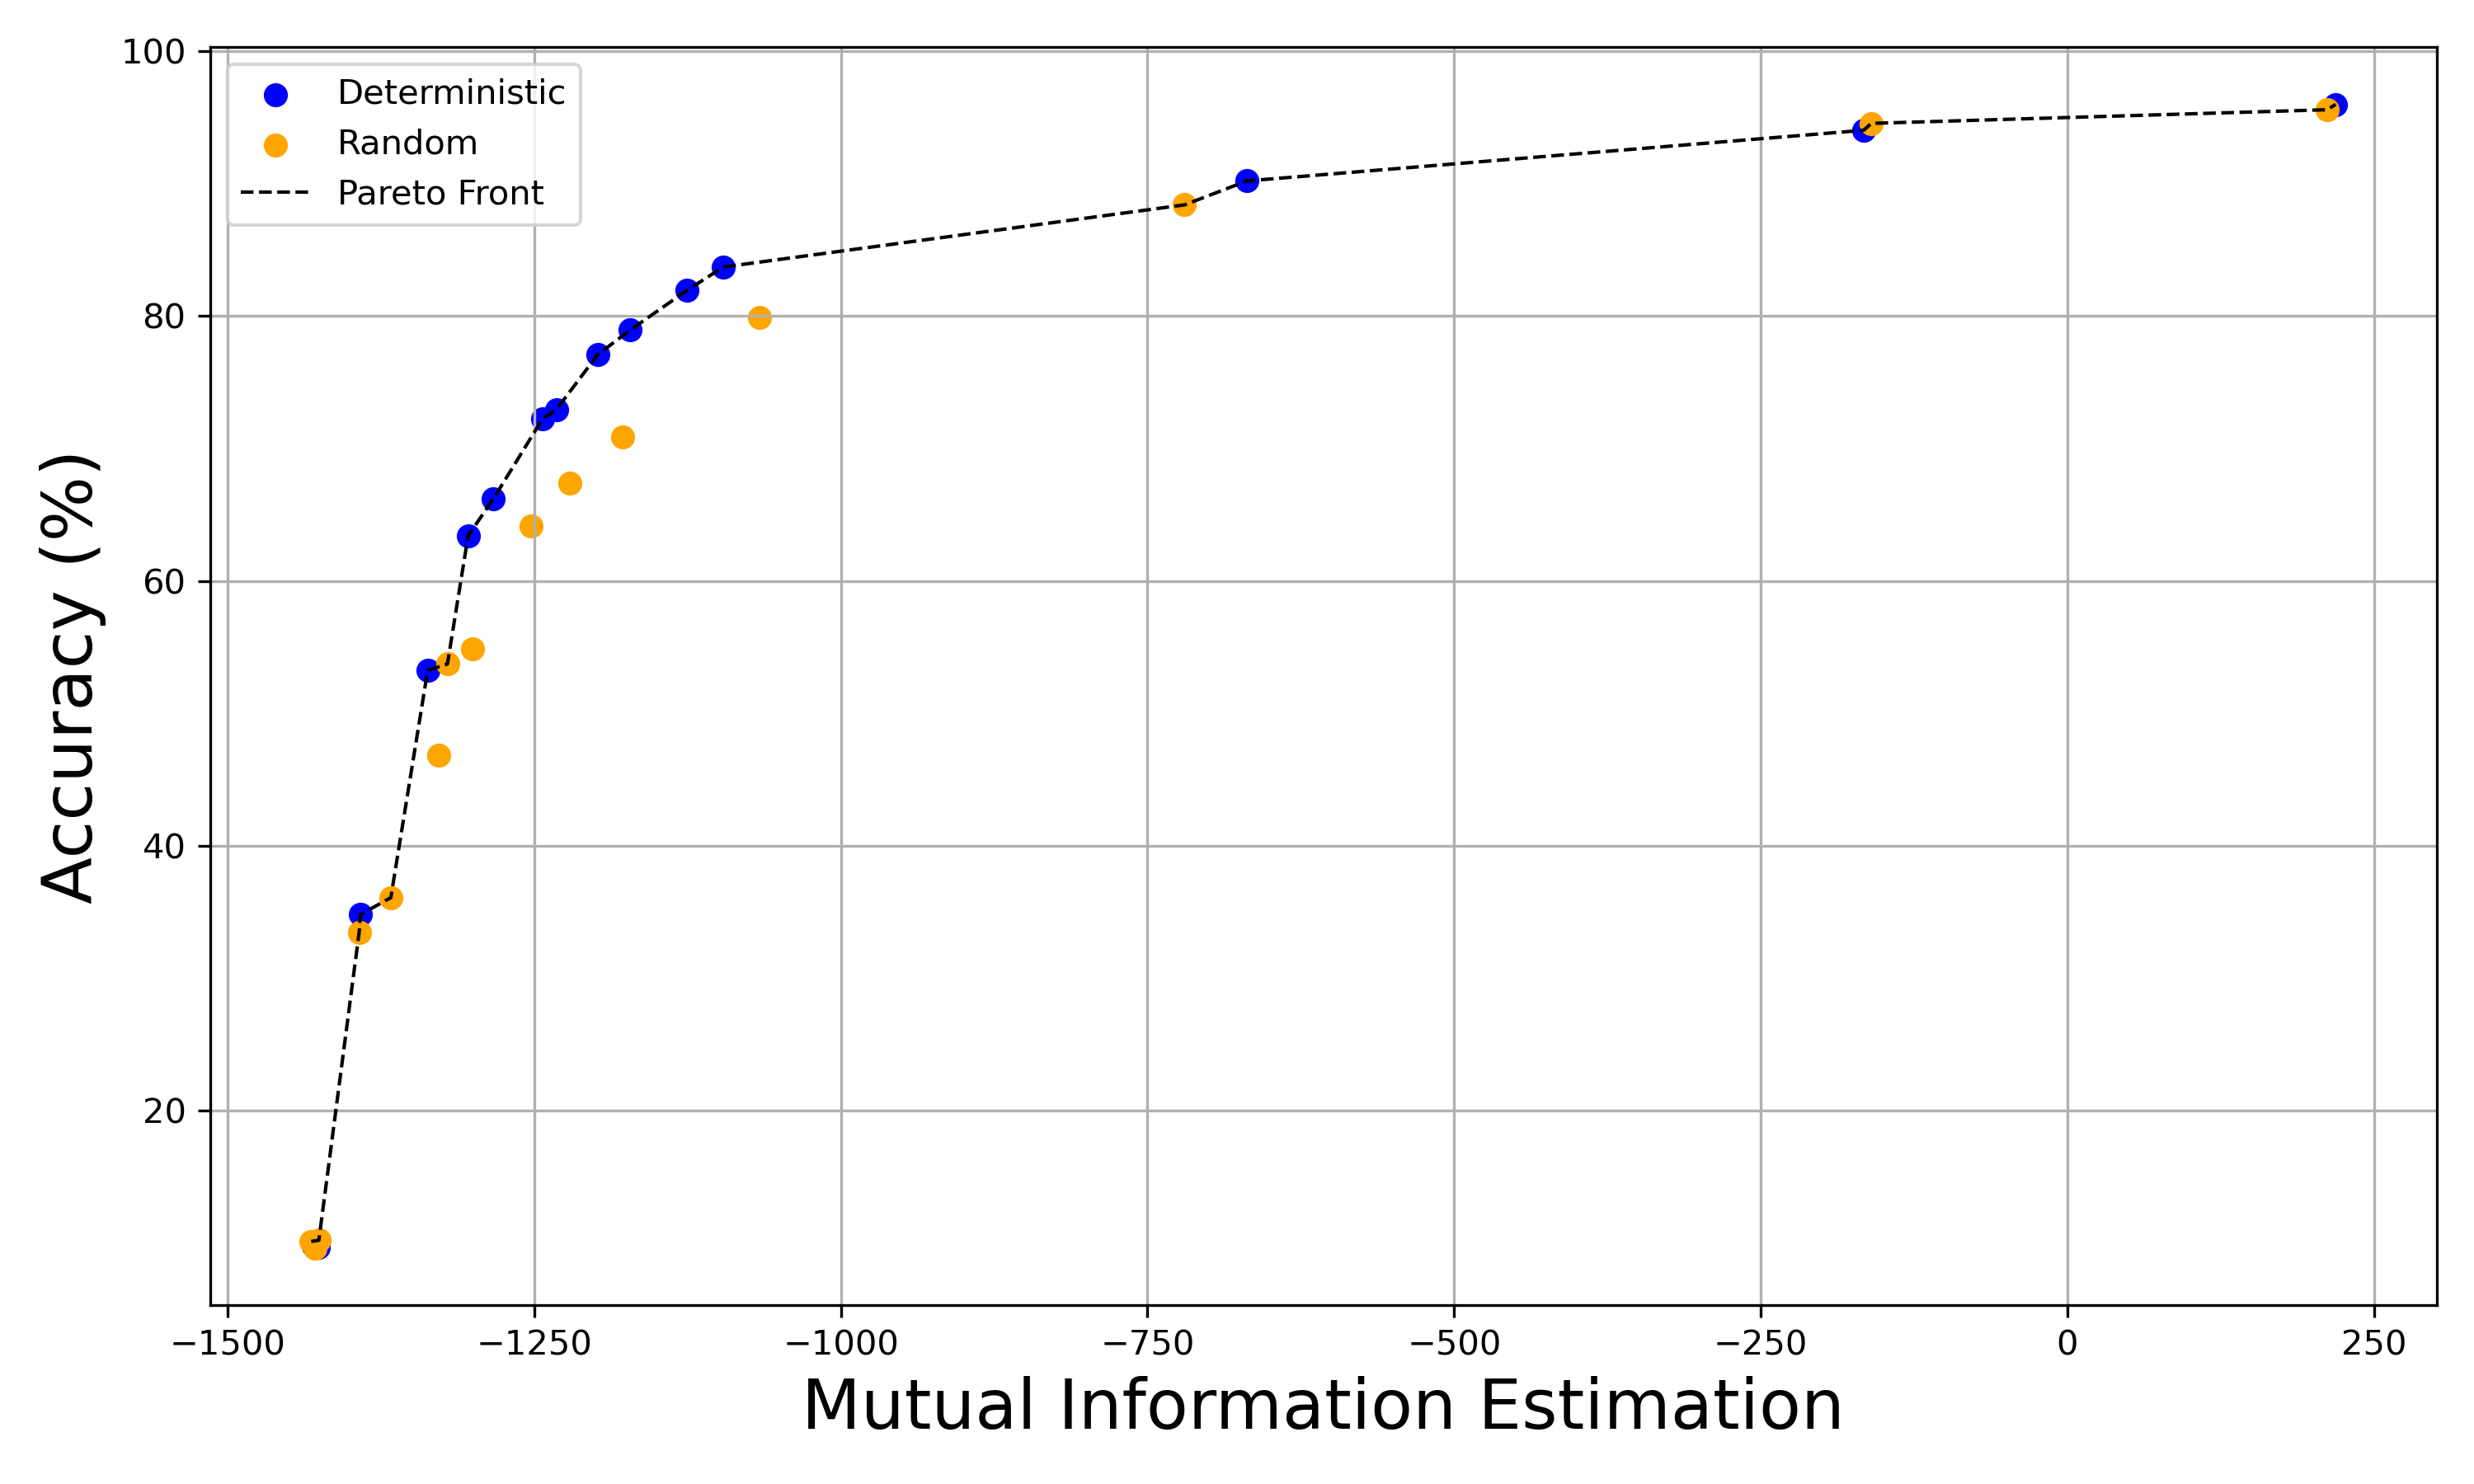
\includegraphics[width=1\textwidth]{conv_pareto_front.png}
    % \caption{\scriptsize .}
\end{figure}
\textbf{Вывод:} Модели учитывающие локальность достигают более высокой точности при заданной взаимной информации, т.е. они лежат на Парето-фронте.
\end{frame}
%----------------------------------------------------------------------------------------------------------
\begin{frame}{Заключение}
\stepcounter{realframenumber}
\textbf{Выносится на защиту}
\begin{enumerate}
    \item Предложен критерий выбора модели для определения индуктивного смещения для заданого множества задач.
    \item Приведены теоретические обоснования для предложенного метода.
    \item Проведены эксперименты, которые показали, что модели с оптимальным соотношением качества, информации и сжатия располагаются на Парето-фронте.
\end{enumerate}
% \noindent\rule{\linewidth}{0.4pt}
\vspace{3mm}
\begin{itemize}
    \item Результаты были доложены на 67-й конференции МФТИ.
    \item Планируется подача работы в рецензируемый журнал.
\end{itemize}
\end{frame}
%----------------------------------------------------------------------------------------------------------
\begin{frame}[plain, noframenumbering]{Источники}
    \nocite{multitask_ind_bias}
    \nocite{cosmo_ind_bias_sym_regression}
    \nocite{Tishby2015DeepLA}
    \nocite{KULUNCHAKOV2017221}
    \bibliographystyle{plain}
    \bibliography{ib_in_model_selection}
\end{frame}
%----------------------------------------------------------------------------------------------------------
\begin{frame}[plain]{Приложение: таблица для окружности}
    \begin{table}[ht!]
        \centering
        \begin{tabular}{|c|c|c|c|c|c|c|}
            \hline
            & \# & Accuracy & \(\text{MSE}_1\) & \(\text{MSE}_2\) & \(\operatorname{I(\mathbf{h}(\mathbf{X}), \mathbf{X})}\) & C \\ \hline
            \multirow{5}{*}{\rotatebox{90}{No reg.}} 
            & 1 & 1.00 & \(4.63 \cdot 10^{-2}\) & \(2.22 \cdot 10^{-2}\) & 2.98 & 22 \\
            & 2 & 1.00 & \(6.52 \cdot 10^{-2}\) & \(3.60 \cdot 10^{-3}\) & 4.20 & 34 \\
            & 3 & 0.82 & \(3.56 \cdot 10^{-2}\) & \(4.68 \cdot 10^{-3}\) & 4.82 & 18 \\
            & 4 & 1.00 & \(2.10 \cdot 10^{-2}\) & \(6.24 \cdot 10^{-3}\) & 2.98 & 43 \\
            & 5 & 0.57 & \(2.62 \cdot 10^{-2}\) & \(3.90 \cdot 10^{-2}\) & 2.13 & 38 \\ \hline
            \multirow{5}{*}{\rotatebox{90}{Reg.}} 
            & 6 & 0.83 & \(4.08 \cdot 10^{-14}\) & \(2.26 \cdot 10^{-15}\) & 1.85 & 12 \\
            & 7 & 0.80 & \(6.36 \cdot10^{-2}\) & \(2.11 \cdot 10^{-2}\) & 1.56 & 16 \\
            & 8 & 0.77 & \(7.14 \cdot 10^{-16}\) & \(1.14\cdot10^{-4}\) & 1.86 & 12 \\
            & 9 & 0.78 & \(6.33 \cdot 10^{-2}\) & \(2.12 \cdot 10^{-2}\) & 1.56 & 16 \\
            & 10 & 0.80 & \(6.57 \cdot 10^{-2}\) & \(2.80 \cdot 10^{-2}\) & 1.86 & 10 \\ \hline
        \end{tabular}
        \caption{Найденные модели и метрики для задачи окружности.}
        \label{circles}
    \end{table}
\end{frame}
%----------------------------------------------------------------------------------------------------------
\begin{frame}[plain, noframenumbering]{Приложение: таблицы для 4-пикселя и авторегрессии}
    \begin{table}[ht!]
        \centering
        \begin{tabular}{|c|c|c|c|c|}
            \hline
             \# & Average accuracy & Average MSE  & \(\operatorname{I(\mathbf{h}(\mathbf{X}), \mathbf{X})}\) & C \\ \hline 
             1 & 0.98 & \(3.5 \cdot 10^{-3}\) & 9.57 & 36 \\
             2 & 0.92 & \(8.19 \cdot 10^{-4}\) & 9.14 & 30 \\
             3 & 0.97 & \(5.96 \cdot 10^{-3}\) & 8.58 & 43 \\
             4 & 0.94 & \(1.67 \cdot 10^{-13}\) & 9.96 & 36 \\
             5 & 0.94 & \(3.93 \cdot 10^{-2}\) & 8.30 & 45 \\ \hline
        \end{tabular}
        \caption{Найденные модели и метрики для 4-пикслея.}
        \label{4-pixels}
    \end{table}
    \begin{table}[ht!]\label{ar}
        \centering
        \begin{tabular}{|c|c|c|c|}
            \hline
             \#Datasets & Models & \(\operatorname{I(\mathbf{h}(\mathbf{X}), \mathbf{X})}\) & C \\ \hline 
             1, 2, 5 & \(p_0 x_t\) & 5.83 & 5 \\
             10 & \(p_0 sin^2(x_t)x_t\) &  3.14 & 18 \\ \hline
        \end{tabular}
        \caption{Найденные модели и метрики для авторегрессии.}
        \label{tab:my_label}
    \end{table}
\end{frame}
%----------------------------------------------------------------------------------------------------------
\begin{frame}[plain, noframenumbering]{Приложение: модели для окружности}
\textbf{Model 1:}
    \begin{align*}
    h_0 &= x_0(x_1 + x_1),\\
    h_1 &= (x_0 + p_0) + x_1,\\
    g_0 &= \bigl(p_1 + h_1^2\,p_0^2\bigr) + p_0(p_1 + p_1)(h_0 + h_0),\\
    g_1 &= p_1\,h_0 + p_1 + h_1p_2,\\
    g_2 &= p_2 + (p_1 + h_0)(h_0\,p_0).
    \end{align*}
    
\textbf{Model 2:}
    \begin{align*}
    h_0 &= (x_0 + p_1)p_0,\\
    h_1 &= \sqrt{x_1^2} + p_2p_0,\\
    g_0 &= \bigl(p_0 + h_0^2\bigr) + \Bigl(p_1^4 + (h_1 + p_0)h_1\Bigr),\\
    g_1 &= h_0^2 + h_1,\\
    g_2 &= p_2h_1 + \sqrt{(h_0 + h_0)^2}.
    \end{align*}
\end{frame}
%----------------------------------------------------------------------------------------------------------
\begin{frame}[plain, noframenumbering]{Приложение: модели для окружности}
    \textbf{Model 3:}
    \begin{align*}
    h_0 &= p_1\bigl(p_2 + p_0 + x_0\bigr),\\
    h_1 &= x_1,\\
    g_0 &= h_1p_0 + \bigl(h_1h_0 + p_2^2\bigr),\\
    g_1 &= h_0^2 + p_0^2 + \bigl(p_1p_2 + p_1\bigr) + p_2h_1^2,\\
    g_2 &= \bigl(p_2 + h_0^2 + \sqrt{h_1^2}\bigr)p_2.
    \end{align*}
    
    \textbf{Model 4:}
    \begin{align*}
    h_0 &= p_2x_0x_1,\\
    h_1 &= x_1 + \bigl(2p_2 + p_0 + x_0 + p_1\bigr),\\
    g_0 &= \bigl(h_0 + p_0 + h_0\bigr)p_0 + h_1^2,\\
    g_1 &= (p_1 + h_0)^4 + p_0p_1h_1,\\
    g_2 &= 2p_1h_1^2 + h_0 + p_2^2.
    \end{align*}
\end{frame}
%----------------------------------------------------------------------------------------------------------
\begin{frame}[plain, noframenumbering]{Приложение: модели для окружности}
    \textbf{Model 5:}
    \begin{align*}
    h_0 &= x_0 + x_1x_0p_1 + x_1 + p_0,\\
    h_1 &= p_2^2,\\
    g_0 &= h_0\bigl(h_0 + p_0\bigr) + \bigl(h_0 + p_0\bigr)^2 + 2h_1,\\
    g_1 &= h_1 + 4p_0^2h_0^2\,p_1^2,\\
    g_2 &= p_1.
    \end{align*}

    \textbf{Model 6:}
    \begin{align*}
    h_0 &= p_1,\\
    h_1 &= x_0^2 + x_1^2,\\
    g_0 &= \bigl(h_0h_1 + 2p_0\bigr)h_1^2 + h_0,\\
    g_1 &= p_0 + \sqrt{h_1} + p_1p_2p_0 + p_0^2p_1 + p_1,\\
    g_2 &= p_0 + \sqrt{h_0^2\sqrt{h_1}}.
    \end{align*}
\end{frame}
%----------------------------------------------------------------------------------------------------------
\begin{frame}[plain, noframenumbering]{Приложение: модели для окружности}
    \textbf{Model 7:}
    \begin{align*}
    h_0 &= \bigl(p_2x_0 + x_1\bigr)^2,\\
    h_1 &= p_1,\\
    g_0 &= h_0 + h_1 + 4h_0^2(h_0 + p_0)^2,\\
    g_1 &= p_2p_1 + \sqrt{h_0}p_1 + p_0,\\
    g_2 &= p_0 + h_0(h_1 + p_2h_0).
    \end{align*}
    
    \textbf{Model 8:}
    \begin{align*}
    h_0 &= x_1^2 + x_0^2,\\
    h_1 &= p_0,\\
    g_0 &= h_1h_0 + p_1\bigl(h_0 + p_1\bigr) + h_0^2p_0^2,\\
    g_1 &= \sqrt{h_0} + h_1,\\
    g_2 &= p_2\bigl(h_0p_0 + p_1 + \sqrt{h_0}\bigr).
    \end{align*}
\end{frame}
%----------------------------------------------------------------------------------------------------------
\begin{frame}[plain, noframenumbering]{Приложение: модели для окружности}
    \textbf{Model 9:}
    \begin{align*}
    h_0 &= p_2,\\
    h_1 &= \bigl(x_1 + x_0p_0\bigr)^2,\\
    g_0 &= \bigl(p_2^2 + p_0\bigr)h_1^2p_2^2 + 2h_1 + p_2,\\
    g_1 &= p_2 + \sqrt{h_1}\bigl(p_2^2 + p_1h_1\bigr),\\
    g_2 &= h_0\sqrt{p_1 + h_1 + h_0^2}.
    \end{align*}
    
    \textbf{Model 10:}
    \begin{align*}
    h_0 &= \bigl(x_1 + x_0\bigr)^2,\\
    h_1 &= p_2,\\
    g_0 &= \bigl(p_1 + h_0\bigr)\bigl(h_1 + p_0 + h_1h_0\bigr) + 2p_1,\\
    g_1 &= \sqrt{h_0}h_1^2 + h_1h_0p_0 + p_1,\\
    g_2 &= h_0p_0 + p_1\bigl(h_1 + p_2\bigr)\sqrt{h_0}.
    \end{align*}
\end{frame}
%----------------------------------------------------------------------------------------------------------
\begin{frame}[plain, noframenumbering]{Приложение: модели для 4-пикселя}
    \textbf{Model 1:}
    \begin{align*}
    h_0 &= x_1p_3 -x_2  - p_5 - x_0,\\
    h_1 &= x_2 p_2 + x_3,\\
    g_0 &= \bigl(h_0 + p_1h_0 - h_1h_0 - \max(h_1,p_0)\bigr)\bigl(\max(h_1h_0,p_4 + h_1) + h_0 + p_4p_1\bigr),\\
    g_1 &= h_0\bigl(p_1(p_4 - h_1) - \max(p_3,h_0)\bigr).
    \end{align*}
    
    \textbf{Model 2:}
    \begin{align*}
    h_0 &= x_1,\\
    h_1 &= \max\bigl(p_4,x_2 - x_0\bigr) + x_2p_5 - x_3,\\
    g_0 &= \max\bigl(h_1,\max(p_5,h_1)\bigr) - \max\bigl(p_3, h_1 p_0\bigr) - h_0 p_2(h_1 - h_0),\\
    g_1 &= \max\bigl(h_1 - p_5 - p_0,p_1\bigr) + p_1 + 2p_3h_0(p_3 + h_1)(p_0 + p_5).
    \end{align*}
\end{frame}
%----------------------------------------------------------------------------------------------------------
\begin{frame}[plain, noframenumbering]{Приложение: модели для 4-пикселя}
    \textbf{Model 3:}
    \begin{align*}
    h_0 &= \bigl(x_1 + p_2\bigr)\bigl(p_3x_3 + p_1x_2\bigr),\\
    h_1 &= x_1 + p_1x_0,\\
    g_0 &= \max\bigl(h_1 + p_0 - p_5h_0, p_5 - p_4\bigr),\\
    g_1 &= -p_4 + p_5 - \max(h_1,h_1) - (h_0 + p_2) + p_0.
    \end{align*}
    
    \textbf{Model 4:}
    \begin{align*}
    h_0 &= x_1p_3 - x_3\bigl(p_0 + x_2\bigr),\\
    h_1 &= x_0 + x_2p_2,\\
    g_0 &= h_0(h_0 + h_1) + (h_0 + p_4) - p_1p_5\max(h_1,h_1),\\
    g_1 &= (p_1p_2 + p_4 + h_0 + h_1)\max\bigl(p_1p_4, \max(h_1h_0,p_4h_0)\bigr).
    \end{align*}
\end{frame}
%----------------------------------------------------------------------------------------------------------
\begin{frame}[plain, noframenumbering]{Приложение: модели для 4-пикселя}
    \textbf{Model 5:}
    \begin{align*}
    h_0 &= p_3\bigl(x_2 - p_4\bigr)\bigl(p_2 + x_0 + x_1\bigr),\\
    h_1 &= x_1\bigl(p_1 - x_3\bigr),\\
    g_0 &= (p_5 - h_0)(p_0 + h_1) - p_4,\\
    g_1 &= \max\bigl(h_0 + h_1,h_0\bigr) + \max\bigl(h_1p_5,p_4\bigr) - \bigl(h_1^2 + p_3\bigr).
    \end{align*}
\end{frame}
\end{document} 
